%========================================
% LESSON CONTENT: Ecuaciones Cuadráticas
%========================================

\lesson{Ecuaciones Cuadráticas}

%========================================
% SECTION 8.1: Definición y Forma Estándar
%========================================
\subsectiontitle{Definición y Forma Estándar}

\begin{definition}
Una \textbf{ecuación cuadrática} es una ecuación que puede escribirse en la forma:
$$ax^2 + bx + c = 0$$
donde $a$, $b$ y $c$ son números reales con $a \neq 0$.

Esta forma se conoce como la \textbf{forma estándar} de una ecuación cuadrática.
\end{definition}

% Visual representation of quadratic equation components
\begin{center}
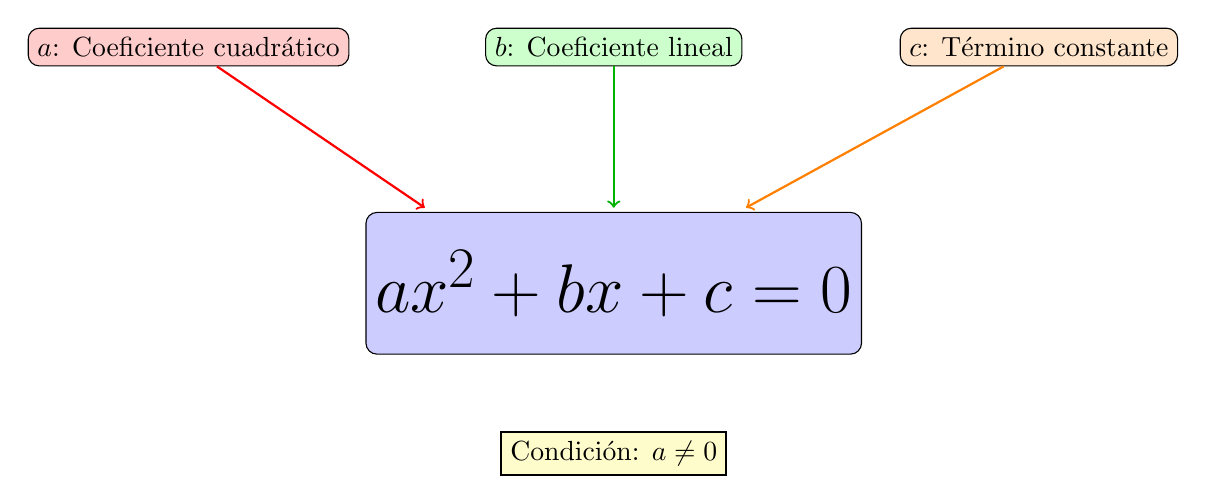
\begin{tikzpicture}[scale=1.2]
    % Central equation box
    \node[draw, fill=blue!20, minimum width=6cm, minimum height=1.8cm, rounded corners] (eq) at (0,0)
        {\Huge $ax^2 + bx + c = 0$};

    % Coefficient labels with color coding
    \node[draw, fill=red!20, rounded corners] (a) at (-4.5,2.5) {$a$: Coeficiente cuadrático};
    \node[draw, fill=green!20, rounded corners] (b) at (0,2.5) {$b$: Coeficiente lineal};
    \node[draw, fill=orange!20, rounded corners] (c) at (4.5,2.5) {$c$: Término constante};

    % Arrows pointing to equation
    \draw[->, thick, red] (a) -- (-2,0.8);
    \draw[->, thick, green!70!black] (b) -- (0,0.8);
    \draw[->, thick, orange] (c) -- (1.4,0.8);

    % Important note
    \node[draw, fill=yellow!20, thick] at (0,-1.8) {Condición: $a \neq 0$};
\end{tikzpicture}
\end{center}

\textbf{Identificación de coeficientes:}

Para identificar correctamente los coeficientes $a$, $b$ y $c$, es esencial escribir la ecuación en forma estándar primero.

\begin{example}
\textbf{Ejemplo 1:} Identifique los coeficientes $a$, $b$ y $c$ en las siguientes ecuaciones cuadráticas:

\textbf{a)} $x^2 + 5x + 6 = 0$

\textbf{Solución:} Ya está en forma estándar: $a = 1$, $b = 5$, $c = 6$

\textbf{b)} $2x^2 - 7x = 4$

\textbf{Solución:} Primero escribimos en forma estándar:
\begin{align}
2x^2 - 7x &= 4\\
2x^2 - 7x - 4 &= 0
\end{align}
Por tanto: $a = 2$, $b = -7$, $c = -4$

\textbf{c)} $3x^2 = 12$

\textbf{Solución:} Forma estándar:
$$3x^2 - 12 = 0$$
Por tanto: $a = 3$, $b = 0$, $c = -12$

\textbf{d)} $-x^2 + 4x + 1 = 0$

\textbf{Solución:} Ya está en forma estándar: $a = -1$, $b = 4$, $c = 1$
\end{example}

%========================================
% SECTION 8.2: Método de Factorización
%========================================
\subsectiontitle{Método de Factorización}

El primer método para resolver ecuaciones cuadráticas se basa en el principio fundamental del producto cero.

\begin{theorem}
\textbf{Principio del Producto Cero (Zero Product Property):}

Si $p$ y $q$ son expresiones algebraicas, entonces:
$$pq = 0 \quad \text{si y solo si} \quad p = 0 \quad \text{o bien} \quad q = 0$$
\end{theorem}

\textbf{Procedimiento para resolver por factorización:}

\begin{enumerate}
\item Escribir la ecuación en forma estándar: $ax^2 + bx + c = 0$
\item Factorizar completamente el lado izquierdo de la ecuación
\item Aplicar el principio del producto cero: igualar cada factor a cero
\item Resolver las ecuaciones lineales resultantes
\item Verificar las soluciones en la ecuación original
\end{enumerate}

% Visual flowchart for factorization method
\begin{center}
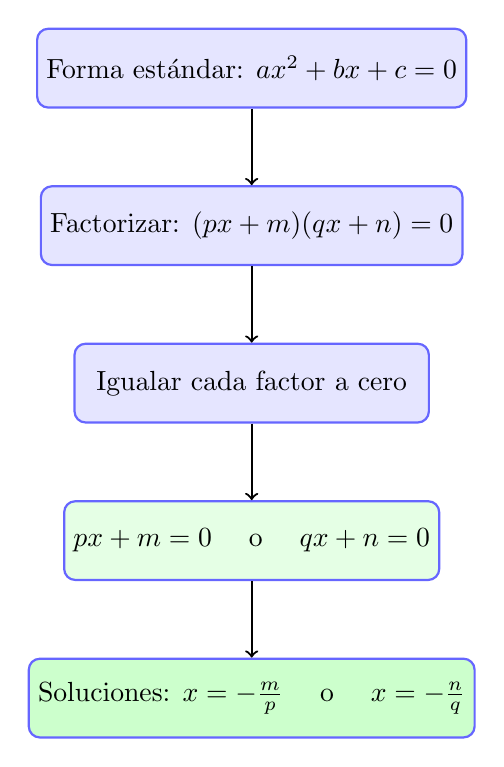
\begin{tikzpicture}[
    stepstyle/.style={rectangle, draw=blue!60, fill=blue!10, thick, minimum width=4.5cm, text centered, minimum height=1cm, rounded corners},
    arrowstyle/.style={->, thick}
]
    \node[stepstyle] (step1) at (0,0) {Forma estándar: $ax^2 + bx + c = 0$};
    \node[stepstyle] (step2) at (0,-2) {Factorizar: $(px + m)(qx + n) = 0$};
    \node[stepstyle] (step3) at (0,-4) {Igualar cada factor a cero};
    \node[stepstyle, fill=green!10] (step4) at (0,-6) {$px + m = 0$ \quad o \quad $qx + n = 0$};
    \node[stepstyle, fill=green!20] (step5) at (0,-8) {Soluciones: $x = -\frac{m}{p}$ \quad o \quad $x = -\frac{n}{q}$};

    \draw[arrowstyle] (step1) -- (step2);
    \draw[arrowstyle] (step2) -- (step3);
    \draw[arrowstyle] (step3) -- (step4);
    \draw[arrowstyle] (step4) -- (step5);
\end{tikzpicture}
\end{center}

\begin{example}
\textbf{Ejemplo 2:} Resuelva $x^2 + 7x + 12 = 0$ por factorización.

\textbf{Solución:}

\textbf{Paso 1:} La ecuación ya está en forma estándar.

\textbf{Paso 2:} Factorizamos el trinomio. Buscamos dos números que multipliquen 12 y sumen 7: estos son 3 y 4.
$$x^2 + 7x + 12 = (x + 3)(x + 4) = 0$$

\textbf{Paso 3:} Aplicamos el principio del producto cero:
$$x + 3 = 0 \quad \text{o bien} \quad x + 4 = 0$$

\textbf{Paso 4:} Resolvemos cada ecuación:
\begin{align}
x + 3 &= 0 \quad \Rightarrow \quad x = -3\\
x + 4 &= 0 \quad \Rightarrow \quad x = -4
\end{align}

\textbf{Respuesta:} Las soluciones son $x = -3$ y $x = -4$.

\textbf{Verificación:} Para $x = -3$: $(-3)^2 + 7(-3) + 12 = 9 - 21 + 12 = 0$ $\checkmark$
\end{example}

\newpage

\begin{example}
\textbf{Ejemplo 3:} Resuelva $6x^2 + x - 12 = 0$ por factorización.

\textbf{Solución:}

Usamos el método AC: $ac = 6(-12) = -72$. Buscamos dos números que multipliquen $-72$ y sumen $1$: estos son $9$ y $-8$.

\begin{align}
6x^2 + x - 12 &= 0\\
6x^2 + 9x - 8x - 12 &= 0\\
3x(2x + 3) - 4(2x + 3) &= 0\\
(2x + 3)(3x - 4) &= 0
\end{align}

Aplicamos el principio del producto cero:
\begin{align}
2x + 3 &= 0 \quad \Rightarrow \quad x = -\frac{3}{2}\\
3x - 4 &= 0 \quad \Rightarrow \quad x = \frac{4}{3}
\end{align}

\textbf{Respuesta:} $x = -\frac{3}{2}$ o $x = \frac{4}{3}$
\end{example}

\begin{example}
\textbf{Ejemplo 4:} Resuelva $x^2 - 9 = 0$ por factorización.

\textbf{Solución:}

Reconocemos una diferencia de cuadrados: $x^2 - 9 = x^2 - 3^2$

\begin{align}
x^2 - 9 &= 0\\
(x + 3)(x - 3) &= 0
\end{align}

Aplicamos el principio del producto cero:
\begin{align}
x + 3 &= 0 \quad \Rightarrow \quad x = -3\\
x - 3 &= 0 \quad \Rightarrow \quad x = 3
\end{align}

\textbf{Respuesta:} $x = -3$ o $x = 3$
\end{example}

\newpage
%========================================
% SECTION 8.3: Método de Completar el Cuadrado
%========================================
\subsectiontitle{Método de Completar el Cuadrado}

El método de completar el cuadrado transforma una ecuación cuadrática en la forma $(x + p)^2 = q$, que se puede resolver fácilmente tomando la raíz cuadrada de ambos lados.

\begin{definition}
\textbf{Completar el cuadrado} es una técnica algebraica que convierte una expresión cuadrática $x^2 + bx$ en un trinomio cuadrado perfecto sumando el término $\left(\frac{b}{2}\right)^2$.
\end{definition}

\textbf{Fórmula clave:}
$$x^2 + bx + \left(\frac{b}{2}\right)^2 = \left(x + \frac{b}{2}\right)^2$$

% Geometric visualization of completing the square
\begin{center}
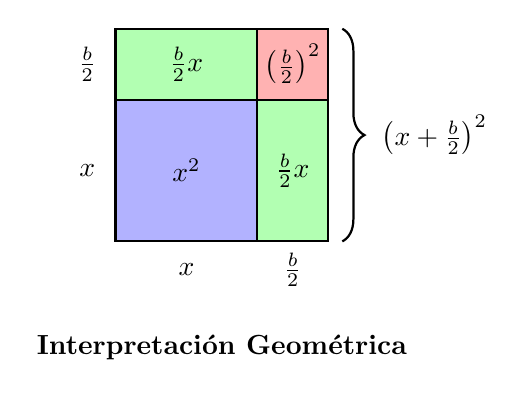
\begin{tikzpicture}[scale=0.9]
    % Original square x^2
    \draw[fill=blue!30, thick] (0,0) rectangle (2,2);
    \node at (1,1) {$x^2$};
    \node at (1,-0.4) {$x$};
    \node at (-0.4,1) {$x$};

    % Added rectangles for bx/2
    \draw[fill=green!30, thick] (2,0) rectangle (3,2);
    \node at (2.5,1) {$\frac{b}{2}x$};
    \node at (2.5,-0.4) {$\frac{b}{2}$};

    \draw[fill=green!30, thick] (0,2) rectangle (2,3);
    \node at (1,2.5) {$\frac{b}{2}x$};
    \node at (-0.4,2.5) {$\frac{b}{2}$};

    % Missing square (b/2)^2
    \draw[fill=red!30, thick] (2,2) rectangle (3,3);
    \node at (2.5,2.5) {$\left(\frac{b}{2}\right)^2$};

    % Bracket showing complete square
    \draw[decorate, decoration={brace, amplitude=8pt, mirror}, thick] (3.2,0) -- (3.2,3);
    \node at (4.5,1.5) {$\left(x + \frac{b}{2}\right)^2$};

    \node at (1.5,-1.5) {\textbf{Interpretación Geométrica}};
\end{tikzpicture}
\end{center}

\textbf{Procedimiento para completar el cuadrado:}

\begin{enumerate}
\item Si $a \neq 1$, dividir toda la ecuación por $a$
\item Mover el término constante al lado derecho
\item Calcular $\left(\frac{b}{2}\right)^2$ y sumar a ambos lados
\item Factorizar el lado izquierdo como un cuadrado perfecto
\item Tomar la raíz cuadrada de ambos lados (recordar el $\pm$)
\item Resolver para $x$
\end{enumerate}

\begin{example}
\textbf{Ejemplo 5:} Resuelva $x^2 + 6x + 5 = 0$ completando el cuadrado.

\textbf{Solución:}

\textbf{Paso 1:} El coeficiente de $x^2$ es 1, continuamos.

\textbf{Paso 2:} Movemos el término constante:
$$x^2 + 6x = -5$$

\textbf{Paso 3:} Calculamos $\left(\frac{6}{2}\right)^2 = 9$ y sumamos a ambos lados:
$$x^2 + 6x + 9 = -5 + 9$$

\textbf{Paso 4:} Factorizamos el lado izquierdo:
$$(x + 3)^2 = 4$$

\textbf{Paso 5:} Tomamos raíz cuadrada:
$$x + 3 = \pm 2$$

\textbf{Paso 6:} Resolvemos:
\begin{align}
x + 3 &= 2 \quad \Rightarrow \quad x = -1\\
x + 3 &= -2 \quad \Rightarrow \quad x = -5
\end{align}

\textbf{Respuesta:} $x = -1$ o $x = -5$
\end{example}

\begin{example}
\textbf{Ejemplo 6:} Resuelva $2x^2 - 8x + 2 = 0$ completando el cuadrado.

\textbf{Solución:}

\textbf{Paso 1:} Dividimos por 2:
$$x^2 - 4x + 1 = 0$$

\textbf{Paso 2:} Movemos el término constante:
$$x^2 - 4x = -1$$

\textbf{Paso 3:} Calculamos $\left(\frac{-4}{2}\right)^2 = 4$ y sumamos a ambos lados:
$$x^2 - 4x + 4 = -1 + 4$$

\textbf{Paso 4:} Factorizamos:
$$(x - 2)^2 = 3$$

\textbf{Paso 5:} Tomamos raíz cuadrada:
$$x - 2 = \pm\sqrt{3}$$

\textbf{Paso 6:} Resolvemos:
$$x = 2 \pm \sqrt{3}$$

\textbf{Respuesta:} $x = 2 + \sqrt{3}$ o $x = 2 - \sqrt{3}$
\end{example}

%========================================
% SECTION 8.4: Fórmula Cuadrática
%========================================
\subsectiontitle{Fórmula Cuadrática}

La fórmula cuadrática es el método más general para resolver ecuaciones cuadráticas. Funciona para cualquier ecuación cuadrática, sin importar si es factorizable o no.

\begin{theorem}
\textbf{Fórmula Cuadrática:}

Las soluciones de la ecuación cuadrática $ax^2 + bx + c = 0$ (con $a \neq 0$) están dadas por:
$$\boxed{x = \frac{-b \pm \sqrt{b^2 - 4ac}}{2a}}$$
\end{theorem}

% Visual breakdown of the quadratic formula
\begin{center}
\begin{tikzpicture}[scale=1]
    % Formula at top
    \node at (0,3.5) {\Huge $x = \dfrac{-b \pm \sqrt{b^2 - 4ac}}{2a}$};

    % Component boxes - reordered: left (-b), middle (2a), right (discriminant)
    \node[draw, fill=blue!20, rounded corners, text width=2.8cm, align=center] (comp1) at (-4.5,0)
        {$-b$\\Opuesto del\\coeficiente lineal};

    \node[draw, fill=red!20, rounded corners, text width=2.8cm, align=center] (comp3) at (0,0)
        {$2a$\\Doble del\\coef. cuadrático};

    \node[draw, fill=green!20, rounded corners, text width=3.2cm, align=center] (comp2) at (4.5,0)
        {$\sqrt{b^2 - 4ac}$\\Raíz del\\discriminante};

    % Arrows pointing to specific parts of the formula
    \draw[->, thick, blue] (comp1.north) -- (-2,3);
    \draw[->, thick, red] (comp3.north) -- (0.6,2.2);
    \draw[->, thick, green!70!black] (comp2.north) -- (2.5,3);

    % Plus-minus symbol note
    \node[draw, fill=yellow!20, rounded corners] at (0,-2) {El símbolo $\pm$ genera dos soluciones};
\end{tikzpicture}
\end{center}

\textbf{Procedimiento para usar la fórmula cuadrática:}

\begin{enumerate}
\item Escribir la ecuación en forma estándar: $ax^2 + bx + c = 0$
\item Identificar los valores de $a$, $b$ y $c$
\item Sustituir en la fórmula cuadrática
\item Simplificar la expresión bajo el radical
\item Calcular ambas soluciones usando $+$ y $-$
\item Simplificar las respuestas
\end{enumerate}

\newpage

\begin{example}
\textbf{Ejemplo 7:} Resuelva $x^2 - 5x + 6 = 0$ usando la fórmula cuadrática.

\textbf{Solución:}

\textbf{Paso 1:} La ecuación está en forma estándar.

\textbf{Paso 2:} Identificamos: $a = 1$, $b = -5$, $c = 6$

\textbf{Paso 3:} Sustituimos en la fórmula:
$$x = \frac{-(-5) \pm \sqrt{(-5)^2 - 4(1)(6)}}{2(1)}$$

\textbf{Paso 4:} Simplificamos:
\begin{align}
x &= \frac{5 \pm \sqrt{25 - 24}}{2}\\
x &= \frac{5 \pm \sqrt{1}}{2}\\
x &= \frac{5 \pm 1}{2}
\end{align}

\textbf{Paso 5:} Calculamos ambas soluciones:
\begin{align}
x_1 &= \frac{5 + 1}{2} = \frac{6}{2} = 3\\
x_2 &= \frac{5 - 1}{2} = \frac{4}{2} = 2
\end{align}

\textbf{Respuesta:} $x = 3$ o $x = 2$
\end{example}

\begin{example}
\textbf{Ejemplo 8:} Resuelva $2x^2 + 3x - 5 = 0$ usando la fórmula cuadrática.

\textbf{Solución:}

Identificamos: $a = 2$, $b = 3$, $c = -5$

\begin{align}
x &= \frac{-3 \pm \sqrt{3^2 - 4(2)(-5)}}{2(2)}\\
x &= \frac{-3 \pm \sqrt{9 + 40}}{4}\\
x &= \frac{-3 \pm \sqrt{49}}{4}\\
x &= \frac{-3 \pm 7}{4}
\end{align}

Calculamos:
\begin{align}
x_1 &= \frac{-3 + 7}{4} = \frac{4}{4} = 1\\
x_2 &= \frac{-3 - 7}{4} = \frac{-10}{4} = -\frac{5}{2}
\end{align}

\textbf{Respuesta:} $x = 1$ o $x = -\frac{5}{2}$
\end{example}

\begin{example}
\textbf{Ejemplo 9:} Resuelva $x^2 + 2x - 4 = 0$ usando la fórmula cuadrática.

\textbf{Solución:}

Identificamos: $a = 1$, $b = 2$, $c = -4$

\begin{align}
x &= \frac{-2 \pm \sqrt{2^2 - 4(1)(-4)}}{2(1)}\\
x &= \frac{-2 \pm \sqrt{4 + 16}}{2}\\
x &= \frac{-2 \pm \sqrt{20}}{2}\\
x &= \frac{-2 \pm 2\sqrt{5}}{2}\\
x &= \frac{2(-1 \pm \sqrt{5})}{2}\\
x &= -1 \pm \sqrt{5}
\end{align}

\textbf{Respuesta:} $x = -1 + \sqrt{5}$ o $x = -1 - \sqrt{5}$
\end{example}

\newpage
%========================================
% SECTION 8.5: El Discriminante
%========================================
\subsectiontitle{El Discriminante}

El discriminante es la expresión que aparece bajo el radical en la fórmula cuadrática. Nos permite determinar la naturaleza de las soluciones sin necesidad de resolverlas completamente.

\begin{definition}
Para una ecuación cuadrática $ax^2 + bx + c = 0$, el \textbf{discriminante} se define como:
$$D = b^2 - 4ac$$
\end{definition}

\begin{theorem}
\textbf{Naturaleza de las raíces según el discriminante:}

Sea $D = b^2 - 4ac$ el discriminante de la ecuación $ax^2 + bx + c = 0$. Entonces:

\begin{itemize}
\item Si $D > 0$: La ecuación tiene \textbf{dos raíces reales distintas}
\item Si $D = 0$: La ecuación tiene \textbf{una raíz real doble} (raíz repetida)
\item Si $D < 0$: La ecuación \textbf{no tiene raíces reales}
\end{itemize}
\end{theorem}

% Table showing discriminant cases
\begin{center}
\begin{tabular}{|c|c|c|c|}
\hline
\textbf{Discriminante} & \textbf{Valor de $D$} & \textbf{Naturaleza} & \textbf{Ejemplo} \\
\hline
$D > 0$ & Positivo & Dos raíces reales distintas & $x^2 - 5x + 6 = 0$ \\
& & & $D = 25 - 24 = 1$ \\
\hline
$D = 0$ & Cero & Una raíz real doble & $x^2 - 4x + 4 = 0$ \\
& & & $D = 16 - 16 = 0$ \\
\hline
$D < 0$ & Negativo & No hay raíces reales & $x^2 + x + 1 = 0$ \\
& & & $D = 1 - 4 = -3$ \\
\hline
\end{tabular}
\end{center}

% Visual representation with parabolas
\begin{center}
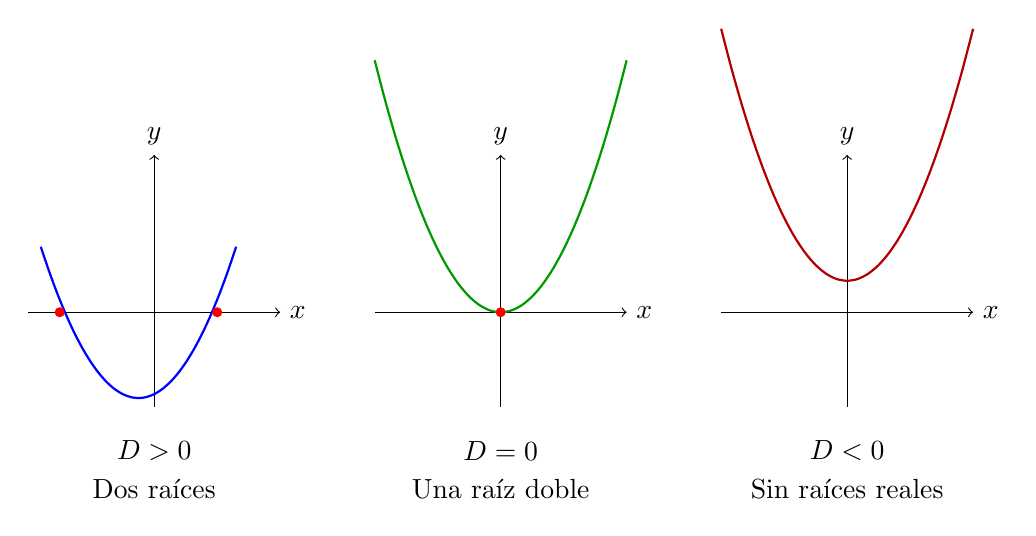
\begin{tikzpicture}[scale=0.8]
    % D > 0 case
    \begin{scope}[xshift=0cm]
        \draw[->] (-2,0) -- (2,0) node[right] {$x$};
        \draw[->] (0,-1.5) -- (0,2.5) node[above] {$y$};
        \draw[domain=-1.8:1.3, smooth, variable=\x, blue, thick] plot ({\x}, {(\x-1)*(\x+1.5)+0.2});
        \filldraw[red] (-1.5,0) circle (2pt);
        \filldraw[red] (1,0) circle (2pt);
        \node at (0,-2.2) {\textbf{$D > 0$}};
        \node at (0,-2.8) {Dos raíces};
    \end{scope}

    % D = 0 case
    \begin{scope}[xshift=5.5cm]
        \draw[->] (-2,0) -- (2,0) node[right] {$x$};
        \draw[->] (0,-1.5) -- (0,2.5) node[above] {$y$};
        \draw[domain=-2:2, smooth, variable=\x, green!60!black, thick] plot ({\x}, {(\x)^2});
        \filldraw[red] (0,0) circle (2pt);
        \node at (0,-2.2) {\textbf{$D = 0$}};
        \node at (0,-2.8) {Una raíz doble};
    \end{scope}

    % D < 0 case
    \begin{scope}[xshift=11cm]
        \draw[->] (-2,0) -- (2,0) node[right] {$x$};
        \draw[->] (0,-1.5) -- (0,2.5) node[above] {$y$};
        \draw[domain=-2:2, smooth, variable=\x, red!70!black, thick] plot ({\x}, {(\x)^2+0.5});
        \node at (0,-2.2) {\textbf{$D < 0$}};
        \node at (0,-2.8) {Sin raíces reales};
    \end{scope}
\end{tikzpicture}
\end{center}

\begin{example}
\textbf{Ejemplo 10:} Sin resolver la ecuación, determine la naturaleza de las raíces:

\textbf{a)} $x^2 - 6x + 9 = 0$

\textbf{Solución:} $a = 1$, $b = -6$, $c = 9$
\begin{align}
D &= b^2 - 4ac\\
D &= (-6)^2 - 4(1)(9)\\
D &= 36 - 36 = 0
\end{align}
Como $D = 0$, la ecuación tiene una raíz real doble.

\textbf{b)} $2x^2 + 5x - 3 = 0$

\textbf{Solución:} $a = 2$, $b = 5$, $c = -3$
\begin{align}
D &= 5^2 - 4(2)(-3)\\
D &= 25 + 24 = 49 > 0
\end{align}
Como $D > 0$, la ecuación tiene dos raíces reales distintas.

\textbf{c)} $x^2 + 2x + 5 = 0$

\textbf{Solución:} $a = 1$, $b = 2$, $c = 5$
\begin{align}
D &= 2^2 - 4(1)(5)\\
D &= 4 - 20 = -16 < 0
\end{align}
Como $D < 0$, la ecuación no tiene raíces reales.
\end{example}

\newpage
%========================================
% SECTION 8.6: Estrategia de Solución
%========================================
\subsectiontitle{Estrategia de Solución y Comparación de Métodos}

Al resolver una ecuación cuadrática, es importante elegir el método más apropiado según la forma de la ecuación.

% Decision tree flowchart
\begin{center}
\begin{tikzpicture}[
    node distance=2cm,
    decision/.style={diamond, draw, fill=yellow!20, text width=3.5cm, text centered, inner sep=2pt, aspect=2},
    block/.style={rectangle, draw, fill=blue!20, text width=3.5cm, text centered, rounded corners, minimum height=1cm},
    result/.style={rectangle, draw, fill=green!30, text width=3cm, text centered, rounded corners},
    arrow/.style={->, thick}
]
    % Start
    \node[block, fill=purple!20] (start) {Ecuación Cuadrática\\$ax^2+bx+c=0$};

    % First decision
    \node[decision, below of=start, yshift=-1cm] (easy) {¿Es fácil de\\factorizar?};

    % Factorization path
    \node[result, below of=easy, yshift=-1.5cm, xshift=-4cm] (factor) {\textbf{Usar Factorización}\\Rápido y directo};

    % Second decision
    \node[decision, below of=easy, yshift=-1.5cm, xshift=4cm] (choose) {¿Qué método\\prefieres?};

    % Formula path
    \node[result, below of=choose, yshift=-1.5cm, xshift=-2.5cm] (formula) {\textbf{Fórmula Cuadrática}\\Siempre funciona};

    % Completing square path
    \node[result, below of=choose, yshift=-1.5cm, xshift=2.5cm] (complete) {\textbf{Completar Cuadrado}\\Útil teóricamente};

    % Arrows
    \draw[arrow] (start) -- (easy);
    \draw[arrow] (easy) -- node[left, near start] {Sí} (factor);
    \draw[arrow] (easy) -- node[above, near start] {No} (choose);
    \draw[arrow] (choose) -- (formula);
    \draw[arrow] (choose) -- (complete);
\end{tikzpicture}
\end{center}

\textbf{Comparación de métodos:}

\begin{center}
\begin{tabular}{|l|c|c|l|}
\hline
\textbf{Método} & \textbf{Velocidad} & \textbf{Aplicabilidad} & \textbf{Cuándo usar} \\
\hline
Factorización & Rápida & Limitada & Cuando se ve factorización obvia \\
\hline
Fórmula Cuadrática & Media & Universal & Cuando no es fácil factorizar \\
\hline
Completar Cuadrado & Lenta & Universal & Para derivar fórmula, análisis \\
\hline
\end{tabular}
\end{center}

\textbf{Recomendaciones generales:}

\begin{enumerate}
\item \textbf{Intenta factorizar primero} si ves patrones obvios (trinomios simples, diferencia de cuadrados)
\item \textbf{Usa la fórmula cuadrática} si la factorización no es evidente
\item \textbf{Calcula el discriminante} primero si solo necesitas saber la naturaleza de las raíces
\item \textbf{Completa el cuadrado} principalmente para propósitos teóricos o cuando se requiere específicamente
\end{enumerate}

%========================================
% SECTION 8.7: Aplicaciones
%========================================
\subsectiontitle{Aplicaciones de Ecuaciones Cuadráticas}

Las ecuaciones cuadráticas aparecen frecuentemente en problemas del mundo real.

\begin{example}
\textbf{Ejemplo 11 (Geometría):} Un rectángulo tiene un largo que es 3 cm mayor que su ancho. Si el área del rectángulo es 40 cm$^2$, encuentre las dimensiones del rectángulo.

\textbf{Solución:}

Sea $x$ = ancho del rectángulo (en cm)

Entonces: $x + 3$ = largo del rectángulo

El área está dada por:
$$\text{Área} = \text{ancho} \times \text{largo}$$
$$40 = x(x + 3)$$
$$40 = x^2 + 3x$$
$$x^2 + 3x - 40 = 0$$

Factorizamos:
$$(x + 8)(x - 5) = 0$$

Soluciones: $x = -8$ o $x = 5$

Como $x$ representa una longitud, debe ser positiva: $x = 5$ cm

\textbf{Respuesta:} Ancho = 5 cm, Largo = 8 cm
\end{example}

\begin{example}
\textbf{Ejemplo 12 (Números):} Encuentre dos números consecutivos cuyo producto sea 132.

\textbf{Solución:}

Sea $x$ = primer número

Entonces: $x + 1$ = número consecutivo

El producto es:
$$x(x + 1) = 132$$
$$x^2 + x = 132$$
$$x^2 + x - 132 = 0$$

Factorizamos:
$$(x + 12)(x - 11) = 0$$

Soluciones: $x = -12$ o $x = 11$

\textbf{Respuesta:} Los números son 11 y 12, o $-12$ y $-11$
\end{example}

\begin{example}
\textbf{Ejemplo 13 (Movimiento):} Un objeto se lanza verticalmente hacia arriba con una velocidad inicial de 64 pies/s. Su altura $h$ (en pies) después de $t$ segundos está dada por:
$$h = -16t^2 + 64t$$

¿En qué tiempo(s) el objeto estará a una altura de 48 pies?

\textbf{Solución:}

Sustituimos $h = 48$:
$$48 = -16t^2 + 64t$$
$$-16t^2 + 64t - 48 = 0$$

Dividimos por $-16$:
$$t^2 - 4t + 3 = 0$$

Factorizamos:
$$(t - 1)(t - 3) = 0$$

\textbf{Respuesta:} El objeto estará a 48 pies en $t = 1$ segundo (subiendo) y $t = 3$ segundos (bajando)
\end{example}

\textbf{Nota final:} Las ecuaciones cuadráticas son fundamentales en muchas áreas de las matemáticas y sus aplicaciones. Dominar los diferentes métodos de solución y saber cuándo usar cada uno es esencial para el éxito en cursos más avanzados.
